\documentclass[11pt]{article}

\usepackage[T1]{fontenc}
\usepackage[utf8]{inputenc}
\usepackage{lmodern}
\usepackage{microtype}
\usepackage[margin=1in]{geometry}
\usepackage{setspace}
\usepackage{amsmath,amssymb,bm}
\usepackage{booktabs}
\usepackage{graphicx}
\usepackage{float}
\usepackage{xcolor}
\usepackage[switch]{lineno}
\usepackage[numbers,sort&compress]{natbib}
\usepackage[hidelinks]{hyperref}
\usepackage[capitalise,noabbrev]{cleveref}

\graphicspath{{figures/}}

\newcommand{\method}{MethylLlama}
\newcommand{\wced}{WCED}
\newcommand{\cpg}{CpG}
\newcommand{\betaval}{$\beta$}

\title{MethylLlama: self-supervised foundation modeling of human DNA methylation profiles}
\author{Netanel Azran}
\date{Working manuscript}

\begin{document}
\maketitle
\linenumbers
\onehalfspacing

\begin{abstract}
DNA methylation is an informative biomarker of disease, tissue identity, and biological age,
but conventional task-specific models do not fully exploit context-dependent regulation across
the methylome or the large volume of public profiles lacking harmonized phenotype labels. Here
we present \method{}, a self-supervised foundation model for human DNA methylation, built on a
Transformer encoder and pretrained without phenotype supervision on 169{,}120 profiles from
diverse tissues and studies, represented at 49{,}156 curated CpG sites. \method{} encodes CpG
identity, quantitative methylation state, and genomic position. We adapt Whole-Cell Expression
Decoding to methylation as the Whole-CpG Encoder--Decoder (WCED), which maps independently
sampled partial views of each profile to global sample representations. Each representation is
trained to reconstruct CpG values excluded from its input, while an InfoNCE objective aligns
representations of the same sample across views. On held-out profiles, \method{} preserved sample
identity across partial measurements and reconstructed withheld methylation values. Frozen
representations captured age- and tissue-associated variation but also substantial study-specific
structure. In chronological-age prediction, a five-model ensemble outperformed matched
MethylGPT and ElasticNet pipelines on a common held-out cohort. These findings support
\method{} as a reusable methylation representation model while identifying cross-study
generalization as an important remaining challenge.

% Internal drafting note (not printed): expand demonstrated downstream breadth before submission.

\end{abstract}

\section{Introduction}

DNA methylation is a covalent epigenetic modification that contributes to transcriptional
regulation, chromatin organization, genome stability, and the maintenance of cellular identity.
At CpG dinucleotides, methylation is commonly quantified as a continuous beta value using
array-based assays that profile hundreds of thousands of loci \citep{Bibikova2011,Pidsley2016}.
The biological meaning of a methylation measurement depends on both genomic and cellular
context: regulatory CpGs can reflect altered gene activity, whereas tissue-specific methylation
programs capture differentiation and cell composition \citep{Jones2012,Roadmap2015}. A
methylation profile therefore represents an integrated molecular state rather than a collection
of independent biomarkers.

The stability of DNA methylation, its accessibility across biological specimens, and its
responsiveness to development, ageing, environmental exposure, and disease have made it a
valuable substrate for biomarker discovery. Epigenetic clocks illustrate this potential. Early
regularized models estimated chronological age across tissues \citep{Horvath2013}, while later
clocks were developed to capture mortality risk, health-related ageing, and the pace of
physiological change \citep{Levine2018,Lu2019,Belsky2022,HigginsChen2022}. These models remain
strong and interpretable predictors, but each is optimized for a predefined endpoint; biological
structure shared across methylation datasets must therefore be learned repeatedly for different
phenotypes.

This task-specific paradigm is poorly matched to the scale and heterogeneity of public
methylation data. Existing profiles span tissues, cohorts, disease states, and array platforms,
while high-quality phenotype labels are available for only a subset of samples and differ among
studies. Moreover, platform-defined CpG panels overlap only partially, so models must often
operate on different subsets of the methylome. Conventional linear predictors perform well when
the endpoint and CpG panel are fixed, but their predominantly additive formulation does not
directly model context-dependent relationships among loci. Deep supervised models can capture
such relationships, yet training a separate model for each application leaves the much larger
unlabelled corpus unused and can generalize poorly from small labelled cohorts. These constraints
motivate a foundation-model strategy that separates large-scale representation learning from
task-specific supervision.

Self-supervised pretraining has enabled reusable representations in language, genomics, and
single-cell transcriptomics \citep{Devlin2019,Ji2021,Yang2022,Cui2024}. In DNA methylation,
MethylGPT established that a Transformer can be pretrained on a large collection of human
methylomes and adapted to biological prediction tasks \citep{Ying2024}. MethylGPT combines
masked CpG prediction with whole-profile reconstruction from a global CLS representation,
thereby encouraging that representation to retain sample-level information. Whole-profile
decoding, however, does not explicitly require the representation of a sample to remain stable
when different CpG subsets are observed, nor does it isolate recovery of loci that were entirely
absent from the encoder input. These properties are important when a pretrained representation
must transfer across incomplete profiles and non-identical measurement panels.

Here we present \method{}, a self-supervised foundation model for human DNA methylation.
\method{} was trained from scratch, without phenotype labels, on 169{,}120 profiles represented
at 49{,}156 curated CpG sites, using the large public methylation resource and CpG panel assembled
for MethylGPT \citep{Ying2024}. Each token combines CpG identity with its quantitative
methylation value. A Transformer encoder integrates these measurements, while genomic-rank
rotary position encoding preserves chromosomal order and a dedicated CLS token provides a
global representation for downstream adaptation \citep{Su2024}.

To learn this representation, we adapt the whole cell expression decoder objective introduced in
BMFM-RNA \citep{Dandala2025} to methylation as the Whole-CpG Encoder--Decoder (WCED). Two
independently sampled partial views are generated from each methylation profile and processed by
a shared encoder. For each view, a decoder predicts the measured profile from the CLS
bottleneck, but the reconstruction loss is evaluated only at valid CpGs excluded from that
encoder input, so the objective cannot be satisfied by copying the input forward. A
complementary response to the same problem is offered by scConcept, which discards feature
reconstruction altogether and pretrains cell representations purely by contrasting disjoint
gene-panel views \citep{Bahrami2025}. We adopt that diagnosis but not that remedy: rather than
replacing reconstruction, we retain it in bottleneck form and add an InfoNCE objective that
aligns CLS representations of the two views from the same profile while distinguishing
representations from different profiles \citep{Oord2018}. WCED therefore applies two distinct
pressures to the same embedding, which must both support recovery of unobserved methylation
values and remain stable across CpG subsets.

We show that independently sampled CpG views preserve sample-specific identity and that the CLS
bottleneck supports accurate reconstruction of CpGs withheld from the encoder. Without phenotype
supervision, the pretrained representation captures substantial age- and tissue-associated
variation, and fine-tuning for chronological-age prediction outperforms both a matched MethylGPT
pipeline and an ElasticNet baseline on a common held-out cohort. At the same time, frozen
representations encode strong study-specific structure, and transfer of age information to
entirely unseen studies is heterogeneous. Together, these results establish \method{} as a
reusable DNA methylation foundation model while identifying cohort heterogeneity as a central
challenge for cross-study generalization.

% Internal drafting note (not printed): add additional completed downstream tasks before submission.

\section{Results}

\subsection{Study design and self-supervised pretraining}

We pretrained \method{} on 169,120 human DNA methylation profiles represented in a shared
vocabulary of 49,156 CpG sites. Pretraining was label-free: neither chronological age nor
tissue, sex, dataset, or disease labels contributed to the objective. Each profile generated
two independently sampled views, each containing 50\% of its measured CpGs. A shared encoder
compressed each view into a 256-dimensional CLS representation, from which a decoder predicted
measured CpGs withheld from that view. A symmetric cross-view contrastive term encouraged the
two CLS representations from the same profile to agree while retaining discrimination between
profiles (Fig.~\ref{fig:study-design}).

We evaluated the pretrained encoder on the AltuMAge-derived collection, which contains 10,988
profiles and 21,368 measured CpGs before age-range filtering and duplicate removal. We used the
original train, validation, and test partition (7,416/1,308/2,264 profiles) only for frozen
representation diagnostics. The supervised age benchmark applied the prespecified age filter
and methylation-fingerprint deduplication, generated five stratified training/validation folds,
and retained a common fixed test set of 2,149 unique sample identifiers for every fold and both model
families. This separation is important: the 2,264-profile split supports in-distribution probes,
whereas all reported fine-tuning and paired-comparison metrics use the filtered and deduplicated
2,149-sample test set.

The pretraining corpus size was confirmed directly from the canonical data header
(169,120 profiles $\times$ 49,156 CpG sites) and partitioned 80/10/10 by a fixed permutation,
leaving 16,912 profiles that were never seen during pretraining and are used for the
reconstruction analyses below. This count should not be conflated with the 154,063 post-QC
figure reported for MethylGPT, whose curation pipeline differs.

\begin{figure}[H]
 \centering
 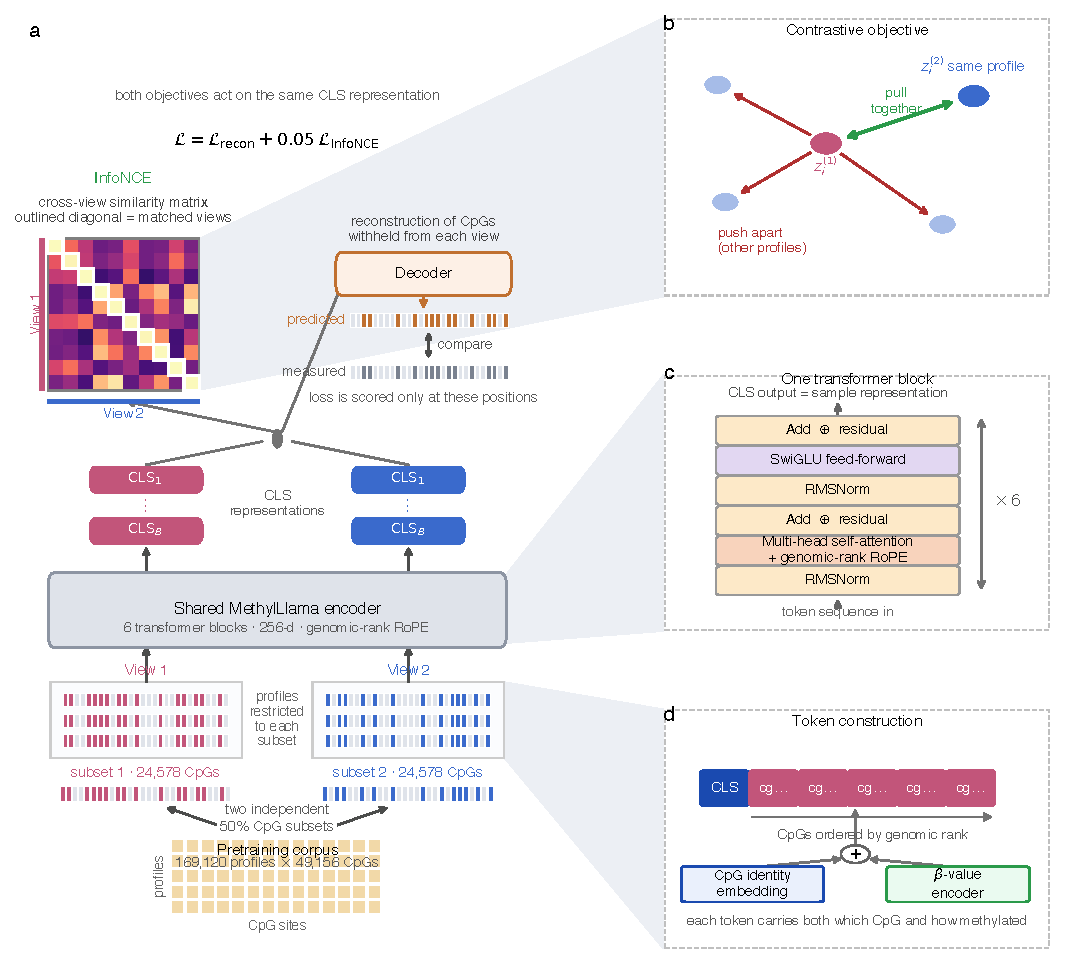
\includegraphics[width=\linewidth]{fig1_study_design_wced.pdf}
 \caption{\textbf{Study design and self-supervised pretraining of \method{}.}
 \textbf{a}, Study design. The unlabelled pretraining corpus is distinguished from the labelled
 AltuMAge evaluation collection, and the two downstream analysis populations are shown
 separately: the 10,988-profile partition used for frozen-representation probes and the
 filtered, deduplicated 2,149-sample test set used for supervised comparisons. Phenotype
 annotations were not used as supervision during pretraining. \textbf{b}, View construction.
 Two independent 50\% subsets of the measured CpGs of one profile form the two views; for each
 view, the complement (hatched) provides the reconstruction target, so the objective is scored
 only at measured CpGs absent from that view. \textbf{c}, The WCED objective. A shared encoder
 maps each view to a CLS representation; a decoder predicts the withheld CpGs from that
 representation alone, and a symmetric InfoNCE term aligns the two projected CLS embeddings.
 \textbf{d}, Token encoding. Each CpG token sums a learned site-identity embedding and a
 continuous $\beta$-value encoding, with a CLS token prepended to every partial profile.}
 \label{fig:study-design}
\end{figure}

\subsection{WCED learns view-consistent global representations}

WCED is designed to compress incomplete observations of a methylation profile into a shared
global representation. Across five independent random draws of two half-profile views for each
of 2,000 profiles, matched views had a mean cosine similarity of $0.984\pm0.0004$, compared
with $0.499\pm0.0002$ for unmatched profiles, and the correct paired view was retrieved for
73.8\% of queries (range 73.1--74.5\% across draws; chance 0.05\%). Retrieval reached 96.1\%
within the ten nearest candidates. The representation is therefore largely invariant to which
half of the methylome is observed while remaining specific enough to identify the individual
profile.

This invariance is nevertheless partly supported by shared input rather than by the
representation alone. Because the two views are drawn independently, they share approximately
half of their CpGs in expectation. Repeating the evaluation with strictly disjoint views---a
random partition in which the two halves share no site---left mean matched similarity almost
unchanged ($0.971\pm0.0005$ versus $0.984$) but reduced top-1 retrieval to
25.3\% (range 24.6--26.0\%). The dissociation is informative: average similarity is insensitive
to the change, whereas identifying the correct partner among 1,999 competitors depends on
narrow margins against the most similar profiles, which the small loss of positive similarity
is sufficient to erase. Cross-subset identity information is clearly retained---disjoint-view
retrieval remains roughly 500-fold above chance, and the correct partner falls within the ten
nearest candidates for 75.1\% of queries, comparable to top-1 performance under overlapping
views---but it is weaker than the overlapping-view figure implies. We note that the encoder was
trained with overlapping views, so disjoint evaluation is out of distribution and these values
are a conservative bound rather than an estimate of what the architecture achieves when trained
for that regime (Supplementary Fig.~S1).

A related question is how far the representation of a partial profile departs from that of the
complete profile, which bears on whether a sample assayed at fewer sites can be embedded
consistently. The embedding of a random 50\% CpG subset had a mean cosine similarity of 0.991
to the embedding of its own complete profile (shuffled-pairing control, 0.496), and a ridge age
probe fitted on complete-profile embeddings and applied without adaptation to subset embeddings
of held-out profiles retained $R^2=0.835$ against $R^2=0.863$ on complete profiles (paired
difference 0.028, 95\% CI 0.014--0.044; Supplementary Fig.~S2). The representation is therefore
substantially, though not perfectly, robust to which half of the measured sites is retained.
We note that these are random subsets rather than the probe set of a particular array
generation, so this does not by itself establish transfer across measurement platforms.

\subsection{WCED reconstructs CpGs withheld from the input}

We evaluated reconstruction on 5,000 profiles from the held-out portion of the pretraining
corpus, encoding each from a 50\% subset of its measured CpGs and scoring predictions only at
measured CpGs absent from that input ($1.12\times10^{8}$ evaluated positions). Predicted and
observed beta values were closely correlated at these withheld sites (Pearson $r=0.972$), and
the per-profile standardized reconstruction loss was 0.0525---closely reproducing the
checkpoint's own validation diagnostics (0.9713 and 0.0552) on profiles excluded from
pretraining (Fig.~\ref{fig:partial-view}c).

To test whether the decoder genuinely reads the sample representation rather than exploiting
population-level regularities, we compared three controls computed on the same profiles under
identical withheld masks. Reconstruction error was 0.0056 for the model, against 0.0306 for a
per-CpG mean predictor, 0.0505 for a decoder given standard normal vectors, and 0.0552 for a
decoder given CLS embeddings shuffled across the batch (Fig.~\ref{fig:partial-view}d). The
model therefore reduced error 5.4-fold relative to the per-CpG mean, even though the mean
predictor was computed on the evaluation cohort itself and is thus advantaged. Notably,
shuffled CLS embeddings produced slightly worse reconstruction than random vectors: supplying
a real but mismatched sample representation is more misleading than supplying no sample
information at all. Together with cross-view consistency, this shows that the CLS bottleneck
carries sample-specific information sufficient both to identify a profile and to predict
methylation values never supplied to that view.

\begin{figure}[H]
 \centering
 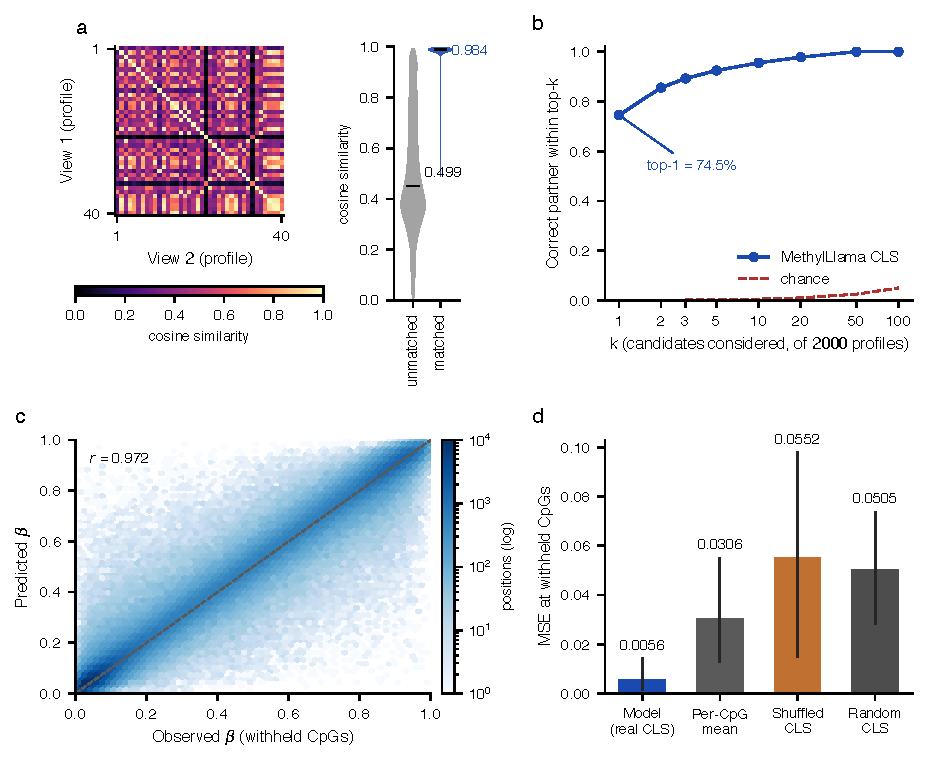
\includegraphics[width=\linewidth]{fig2_wced_consistency_reconstruction.pdf}
 \caption{\textbf{WCED learns consistent partial-view representations and reconstructs
 withheld CpGs.} \textbf{a}, Cosine similarity between CLS embeddings of two independently
 sampled 50\%-CpG views, for 40 representative profiles (heatmap; the bright diagonal marks
 matched views of the same profile) and summarised over all 2,000 profiles (violins; means
 annotated). \textbf{b}, Cross-view retrieval accuracy as a function of the number of
 candidates considered, against chance; the strictest point, top-1, is annotated. Panels a and
 b show one representative draw of two views per profile; values across five independent draws
 are given in the text and in Supplementary Fig.~S1. \textbf{c}, Observed
 versus predicted $\beta$ values at CpGs withheld from the encoder input, for 5,000 profiles
 from the held-out portion of the pretraining corpus (hexagonal binning, logarithmic colour
 scale; dashed line indicates identity). For legibility the panel displays a random subsample
 of $5.0\times10^{5}$ of the $1.12\times10^{8}$ evaluated positions; the reported correlation
 ($r=0.972$) was computed over all evaluated positions, not over the plotted subsample.
 \textbf{d}, Mean squared error at withheld CpGs for the model and three controls evaluated on
 the same profiles under identical withheld masks. Bars show the mean across profiles and
 vertical lines span the 10th--90th percentile across profiles; these are dispersion ranges,
 not confidence intervals.}
 \label{fig:partial-view}
\end{figure}

\subsection{Pretraining captures age and tissue variation}

We next asked whether self-supervised pretraining preserved information useful beyond its
reconstruction objective. A ridge regressor fitted to frozen pretrained CLS embeddings on the
original train-plus-validation profiles achieved $R^2=0.866$ and a median absolute error
(MedAE) of 5.17 years on the original 2,264-profile test split. Applying the same probe to
mean-pooled contextual CpG embeddings reduced performance to $R^2=0.795$ and MedAE 6.53 years.
The CLS space also had a higher effective rank than the mean-pooled space (18.12 versus 3.40)
and lower mean cosine anisotropy (0.500 versus 0.867). These findings indicate that the explicit
sample token retained broader, more age-informative variation than uniform pooling across CpG
tokens, despite receiving no age supervision during pretraining.

Biological information was not restricted to age. A linear classifier trained on frozen CLS
embeddings attained balanced accuracy 0.936 across 37 sufficiently represented tissue classes
(chance level 0.027). These probes establish that biologically associated structure is
accessible in the pretrained representation under an in-distribution sample split. They do not
show that the representation has separated biology from study or platform effects, because
profiles from the same study can occur on both sides of the probe split.

An archived nonlinear replica-head probe reached $R^2=0.922$ and MedAE 3.57 years, but we treat
it as exploratory: the current analysis script does not seed its NumPy minibatch shuffling and
does not reserve a separate split for head-hyperparameter selection. The deterministic ridge
probe is therefore the primary evidence for label-free age information.

\subsection{Age prediction is stable across folds}

We fine-tuned five models using different stratified training/validation folds and evaluated
every selected checkpoint on the same 2,149-sample test set (age range 0--103 years; mean
45.53 years). Across folds, mean MedAE was $3.169\pm0.040$ years, mean MAE was
$4.493\pm0.059$ years, and mean $R^2$ was $0.9316\pm0.0024$ (mean $\pm$ sample SD;
Table~\ref{tab:folds}). The narrow ranges across folds show that performance was not driven by
one favorable supervised partition. Because the test samples were shared, however, these
standard deviations measure training-partition stability and are not confidence intervals for
population performance.

Averaging the five predictions for each sample produced the primary \method{} estimate, with
MedAE 3.112 years, MAE 4.333 years, and $R^2=0.9365$. MethylGPT was aggregated in the same way
for the paired neural-model comparison below.

\begin{table}[H]
\centering
\caption{\textbf{Five-fold stability on the common held-out test set.}
Values were recomputed from saved sample-level predictions. Because every model was evaluated
on the same test samples, fold dispersion quantifies sensitivity to the training partition and
is not a population confidence interval.}
\label{tab:folds}
\begin{tabular}{lrrr}
\toprule
Model & MedAE (years) & MAE (years) & $R^2$ \\
\midrule
Fold 0 & 3.126 & 4.439 & 0.9321 \\
Fold 1 & 3.213 & 4.458 & 0.9337 \\
Fold 2 & 3.209 & 4.570 & 0.9284 \\
Fold 3 & 3.152 & 4.541 & 0.9298 \\
Fold 4 & 3.144 & 4.455 & 0.9338 \\
\midrule
Mean $\pm$ SD & $3.169\pm0.040$ & $4.493\pm0.059$ & $0.9316\pm0.0024$ \\
Fold ensemble & 3.112 & 4.333 & 0.9365 \\
\bottomrule
\end{tabular}
\end{table}

\subsection{\method{} improves age prediction over MethylGPT}

We performed a paired comparison using identical held-out samples, age labels, and fold
assignments for both model families. Fold-level predictions were averaged within sample, and
uncertainty was estimated by resampling the same test samples for both models. \method{}
reduced ensemble MedAE from 3.70 to 3.11 years (paired difference, 0.59 years; 95\% CI,
0.34--0.81) and MAE from 5.11 to 4.33 years, while increasing $R^2$ from 0.911 to 0.936.
Paired confidence intervals for all three endpoints excluded zero
(Fig.~\ref{fig:age-benchmark}).

We additionally evaluated a conventional linear reference using ElasticNetCV
\citep{Zou2005}. Hyperparameters were selected by internal cross-validation on the pooled
training and validation profiles, with the common test set withheld until final evaluation.
The resulting model used 1,036 non-zero coefficients among 21,368 CpGs and achieved MedAE
3.44 years, MAE 4.73 years, and $R^2=0.9322$. The \method{} ensemble therefore had better
point estimates than both ElasticNet and MethylGPT on this test set. Because ElasticNet was
evaluated as a single fitted model and its sample-level predictions were not retained, this
comparison is descriptive and is not assigned a paired confidence interval.

The benchmark is matched at the sample and split levels, but the pipelines differ in their
treatment of 1,760 CpGs outside the shared pretraining reference: \method{} retains their
measured values under a common unknown-CpG identity, whereas MethylGPT excludes them. The
result therefore establishes a predictive advantage for the implemented \method{} pipeline,
but does not attribute that advantage to WCED alone.

\begin{table}[H]
\centering
\caption{\textbf{Age-prediction performance on the common held-out test set.}
The first three rows are test-set point estimates. \method{} and MethylGPT are five-fold
prediction ensembles; ElasticNetCV is a single model selected by internal cross-validation.
The final row reports the paired MethylGPT-minus-\method{} difference and its 95\% bootstrap
confidence interval; positive error differences and a negative $R^2$ difference favor
\method{}.}
\label{tab:age-benchmark}
\small
\begin{tabular}{@{}lccc@{}}
\toprule
Model or comparison & MedAE (years) & MAE (years) & $R^2$ \\
\midrule
\method{} & 3.112 & 4.333 & 0.9365 \\
ElasticNetCV & 3.437 & 4.731 & 0.9322 \\
MethylGPT & 3.701 & 5.105 & 0.9110 \\
\midrule
MethylGPT $-$ \method{} & $0.589\ [0.338,\,0.815]$ &
$0.773\ [0.583,\,0.968]$ & $-0.0254\ [-0.0329,\,-0.0183]$ \\
\bottomrule
\end{tabular}
\end{table}

\begin{figure}[H]
 \centering
 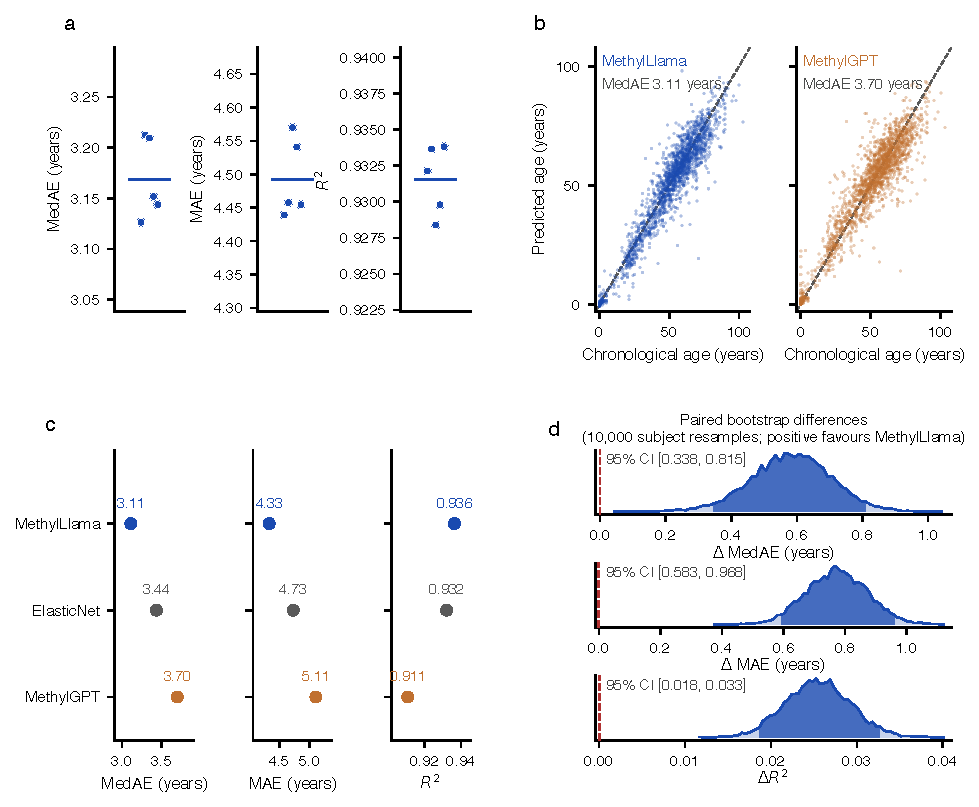
\includegraphics[width=\linewidth]{fig3_age_benchmark_paired_comparison.pdf}
 \caption{\textbf{Stable age prediction and comparison with neural and linear references.}
 \textbf{a}, Test-set MedAE, MAE, and $R^2$ for the five independently fine-tuned \method{}
 folds; horizontal lines denote fold means. \textbf{b}, Ensemble-predicted versus chronological
 age for \method{} and MethylGPT on the same 2,149 held-out samples; each point is one
 sample and dashed lines indicate identity. \textbf{c}, Ensemble point estimates for
 \method{} and MethylGPT and the single-model ElasticNetCV reference. \textbf{d}, Sampling
 distributions of the paired difference between models over 10,000 sample resamples, with the
 central 95\% shaded; error reductions are MethylGPT-minus-\method{} differences, whereas the
 $R^2$ effect is \method{}-minus-MethylGPT, so positive values favor \method{} throughout. The
 vertical dashed lines mark no difference.}
 \label{fig:age-benchmark}
\end{figure}

\subsection{Genomic RoPE induces contextual CpG locality}

To test the representational effect of genomic RoPE, we trained a matched pilot pair on the
same fixed 5,000-profile subset. The two runs used the same architecture, objective, and
hyperparameters; the intentional difference was whether RoPE received genomic-rank positions
or sequential positions. For the genomic-RoPE model, mean cosine similarity of contextualized
representations was 0.9831 for adjacent CpGs and 0.8857 for random pairs, giving a locality gap
of 0.0974. Without genomic positions, the corresponding values were 0.9931 and 0.9621, a gap
of 0.0310. Thus, relative separation of adjacent from random CpGs was approximately 3.14-fold
larger with genomic positions. In the production model's static token-embedding table, adjacent
and random CpGs showed no positive locality gap, consistent with locality emerging through
contextual computation rather than simple clustering of identity embeddings.

This ablation supports a mechanistic interpretation but remains a pilot. It used one seed, and
the selected genomic checkpoint also had better reconstruction diagnostics than the non-genomic
checkpoint (normalized reconstruction loss 0.0906 versus 0.1585; Pearson correlation 0.9357
versus 0.9017). We therefore report the locality result in the Supplementary Results and do not
claim a downstream predictive advantage for genomic RoPE until replicated pretraining runs and
a matched downstream ablation are available.

\subsection{Pretrained representations retain tissue and study structure}

Although tissue was highly predictable from frozen CLS embeddings, study identity was even
more readily accessible: a linear probe attained balanced accuracy 0.956 across 85 eligible
datasets, compared with a chance level of 0.012. Two-dimensional projections likewise formed
many compact study-associated islands. This finding is not evidence of batch invariance.
Instead, it shows that the representation simultaneously retains biological tissue structure
and substantial cohort-specific structure. Tissue and dataset labels are also partially
confounded in public methylation collections, so the tissue-probe accuracy cannot be interpreted
as a study-independent biological metric.

For this reason, the main representation figure should pair the tissue result with the dataset
result rather than show tissue alone. UMAP panels are descriptive and belong in the
Supplementary Information; balanced-accuracy probes and cross-study tests provide the
quantitative evidence (Fig.~\ref{fig:representation-generalization}).

\subsection{Cross-study transfer of age representations remains limited}

We assessed whether age information in frozen CLS embeddings transferred to studies excluded
from probe fitting. Whereas a random-split ridge probe achieved $R^2=0.856$, the median
leave-one-dataset-out $R^2$ across 11 eligible studies was 0.261, with a median MedAE of
8.32 years; three studies yielded negative $R^2$. The broad variation between cohorts shows
that readily decodable age information within a mixed-study split does not ensure robust
transfer to an unseen study.

The failures are not explained by the obvious cohort descriptors. Neither the age dispersion
of the held-out cohort (Spearman $\rho=+0.28$, $P=0.40$) nor its sample size
($\rho=+0.26$, $P=0.43$) was associated with transfer success, and the failing studies overlap
the succeeding ones on both axes: one cohort of 118 profiles with an age SD of 10.5 years
transferred at $R^2=0.42$, whereas a larger cohort of 282 profiles with a wider age SD of
13.9 years transferred at $R^2=-4.63$ (Fig.~\ref{fig:representation-generalization}c). Cohort
size and age range therefore do not account for the heterogeneity, which instead points toward
study-specific biological or technical structure of the kind quantified above.

This is a diagnostic of the frozen representation, not a generalization test of the fully
fine-tuned age model. Differences in tissue, disease status, platform, and age distribution
also remain entangled with study identity. Claims of study-independent age prediction will
therefore require grouped study-held-out fine-tuning with cohort-level uncertainty; the
current analysis identifies cross-study transfer as an unresolved limitation.

\begin{figure}[H]
 \centering
 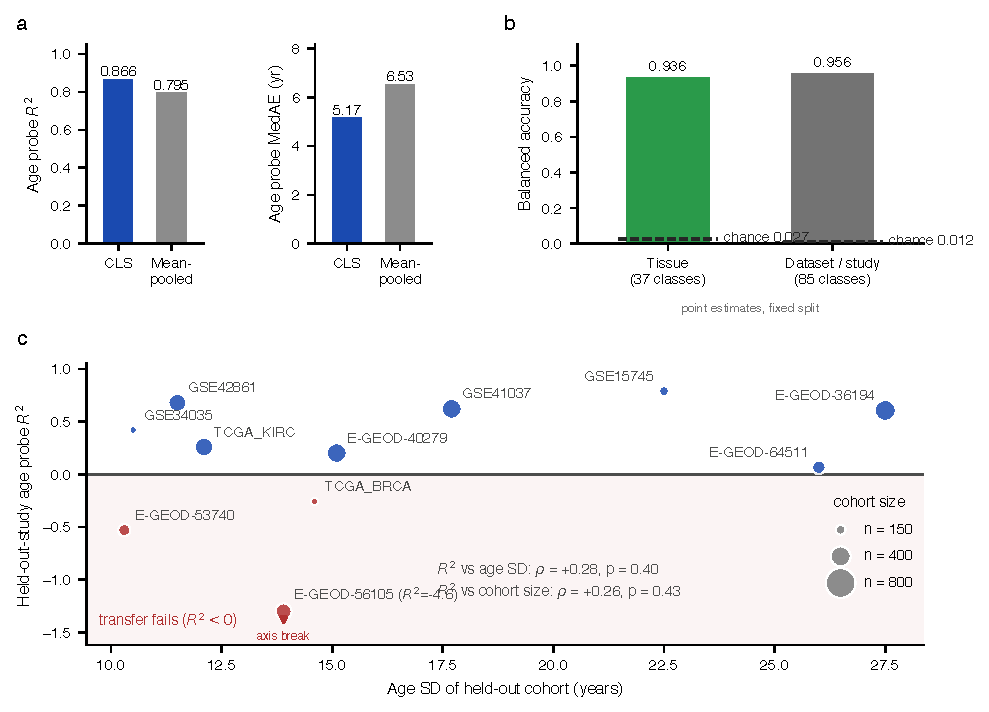
\includegraphics[width=\linewidth]{fig4_representation_cross_study_transfer.pdf}
 \caption{\textbf{Biological structure, study structure, and the limits of cross-study
 transfer.} \textbf{a}, Frozen linear age-probe performance using the pretrained CLS
 representation or mean-pooled contextual CpG embeddings. \textbf{b}, Balanced accuracy of
 frozen CLS linear probes for tissue and dataset/study identity; dark-grey dashed horizontal
 segments mark chance levels. \textbf{c}, Leave-one-dataset-out age-probe $R^2$ for the 11 studies meeting
 the prespecified size ($n\geq100$) and age-dispersion (SD $\geq10$ years) thresholds, plotted
 against the age spread of the held-out cohort, with marker area proportional to cohort size.
 Studies with negative $R^2$ are shown in red on a shaded background; the most extreme value is
 clipped for readability and annotated with its true value. Neither cohort descriptor predicts
 transfer success (Spearman $\rho$ inset). These analyses diagnose the frozen representation and
 do not constitute external validation of the fully fine-tuned model.}
 \label{fig:representation-generalization}
\end{figure}

\section{Discussion}

We developed a partial-view self-supervised framework for learning global representations of
DNA methylation samples. Unlike objectives that operate only at the level of masked features,
WCED routes reconstruction through a CLS bottleneck and evaluates reconstruction at CpGs not
provided to the encoder. Contrastive view matching directly trains the same sample embedding
that is subsequently transferred to downstream analysis. The combination targets a distinction
that is easy to miss in high-dimensional molecular modeling: successful prediction of masked
features is not equivalent to learning a useful global representation.

The current results establish three narrow but meaningful points. First, the encoder can
compress a partial methylation profile while retaining information about unobserved sites.
Second, independently sampled views of the same profile remain identifiable in representation
space. Third, the resulting encoder can be adapted reproducibly to age prediction. The CLS
representation contained age-associated information before fine-tuning and retained more
usable variation than mean pooling, consistent with the intended sample-level bottleneck.

The paired benchmark establishes better predictive performance for the implemented
\method{} pipeline than for MethylGPT on the matched held-out samples. It does not, however,
isolate the source of that difference: the pipelines vary in architecture, optimization, and
their handling of 1,760 CpGs outside the shared pretraining reference. ElasticNet provided a
strong non-neural reference, with performance close to the \method{} ensemble. Although all
three point estimates favored \method{}, sample-level ElasticNet predictions were not retained,
so statistical uncertainty is currently available only for the paired MethylGPT comparison.
Matched objective and initialization ablations are still required before attributing the
downstream gain specifically to WCED or to self-supervised pretraining.

The strongest limitation is cohort structure. Dataset identity is highly recoverable from the
pretrained embeddings, showing that study- or batch-specific signals remain prominent. Random
sample partitions can therefore overestimate transfer when samples from the same source study
appear in model development and evaluation. This issue also changes how representation
visualizations should be read. Separation by tissue may reflect genuine biology, but clean
clusters can coexist with strong study effects. Quantitative study-held-out tests should carry
more evidential weight than visually distinct UMAP clusters.

The representation analyses are therefore best viewed as diagnostics. Attention concentration,
genomic locality, and CpG embedding structure can motivate hypotheses, but they do not by
themselves identify causal age-associated loci or establish biological mechanism. Stronger
interpretation would require stability across folds and seeds, perturbation-based importance,
enrichment against a prespecified CpG background, and correction for multiple testing.

Further limitations include reliance on array-selected CpGs, incomplete evaluation across
platforms, a single firmly established downstream phenotype, and no prospective clinical
validation. A broad foundation-model claim would require transfer across multiple tasks and
cohorts. At the present stage, ``self-supervised methylation encoder'' or ``methylation
representation model'' more precisely describes the demonstrated scope.

In summary, the evidence supports WCED as a method for learning partial-view-consistent global
methylation representations and supports \method{} as a stable age-prediction encoder on the
held-out evaluation set. Whether the objective improves upon matched alternatives and whether
the representation transfers to unseen studies remain the decisive experiments for the final
manuscript.

% Internal drafting note (not printed): Human review: after the controlled comparisons are
%   complete, rewrite the opening and closing Discussion paragraphs around one
%   experimentally attributable conclusion. If no significant pretraining benefit is found,
%   present the paper as an objective evaluation of sample-level bottleneck learning rather
%   than forcing a superiority narrative.

% Ported from the chapter-review draft: all VERIFY/COMPLETE markers resolved
% against checkpoint configs and dataset headers (see git history).
\section{Methods}

\subsection{Datasets and study design}

Self-supervised pretraining used 169,120 public methylation profiles represented over 49,156
CpG sites. Profiles were partitioned once into training, validation, and held-out portions
(80/10/10) by a fixed random permutation (seed 42); the held-out portion of 16,912 profiles
was never seen during pretraining and provides the evaluation set for the reconstruction
analyses reported below. The downstream age corpus was derived from the AltuMAge collection
\citep{deLimaCamillo2022} and comprised 10,988 profiles over 21,368 CpG sites, spanning 37
tissue categories and 85 source studies. After removing 328 profiles with implausible age
annotations ($<0$ or $>120$ years) and 71 duplicate profiles, 10,589 remained: 7,177 training,
1,263 validation, and a common held-out test set of 2,149 unique samples. Because the same
test samples were evaluated by all five fold-trained models, variation across models is
reported as training-fold stability rather than as an independent population confidence
interval.

\paragraph{Split integrity.}
Partitions were defined at the level of individual profiles, indexed by their public sample
accession; donor-level grouping was not available for the majority of source studies, which we
note as a limitation. Duplicate and technical-replicate profiles were identified by
methylation fingerprinting across all partitions, yielding 77 duplicate pairs spanning 136
profiles; within each connected component of the resulting graph the lexicographically first
accession was retained and the remaining 71 profiles were excluded. The same exclusion list
and age filter were applied identically to every model and baseline evaluated here, and set
equality of the resulting 2,149 test accessions was verified programmatically rather than
inferred from matching counts. Exact split manifests and their hashes will accompany the
release.

\paragraph{Preprocessing.}
Beta values were restricted to $[0,1]$. Pretraining used the full 49,156-CpG reference panel;
downstream modelling used the 21,368 CpGs measured in the AltuMAge collection. Missing
measurements were excluded from view sampling and from all loss terms through an explicit
validity mask, so that no imputed value ever contributed to training or evaluation. CpGs were
ordered by chromosome and genomic coordinate on the hg38 assembly using the Illumina HM450
manifest. No target-age labels were used during self-supervised pretraining: although the
implementation exposes an optional auxiliary age-regression term, its weight was set to zero
for the pretraining run reported here.

\subsection{Input representation and encoder}

Each observed CpG was represented by its site identity $c_i$ and beta value $b_i$. The token
embedding was
\begin{equation}
  \bm{x}_i = s_c\,\bm{e}_{c_i} + f_{\beta}(b_i),
\end{equation}
where $\bm{e}_{c_i}$ is a learned CpG embedding, $s_c$ is a learned or initialized scale, and
$f_{\beta}$ is a continuous-value encoder based on sinusoidal basis functions followed by a
linear projection. A CLS token was prepended to every partial profile.

The encoder used six transformer layers with hidden size 256, four attention heads (head
dimension 64), feed-forward width 512, and a vocabulary of 49,161 entries (49,156 CpG sites
plus five special tokens). Transformer blocks used
pre-normalization with RMSNorm \citep{Zhang2019}, multi-head self-attention
\citep{Vaswani2017}, SwiGLU feed-forward layers, and rotary position embeddings
\citep{Su2024,Touvron2023}. RoPE position identifiers were assigned using genomic rank rather
than arbitrary input order. The pooled CLS output served as the sample representation.

\subsection{Partial-view WCED pretraining}

WCED adapts the Whole-Cell Expression Decoder introduced for transcriptomic foundation models
\citep{Dandala2025} to array-derived DNA methylation. The original objective reconstructs a
whole-cell expression profile through a CLS bottleneck; our formulation reconstructs CpG
methylation values and evaluates reconstruction only at sites excluded from the encoder input.

The paired-view design was inspired by scConcept, which contrasts representations of different
gene-panel views of the same cell \citep{Bahrami2025}. For each methylation profile, two
independently sampled views $V_i^{(1)}$ and $V_i^{(2)}$ contained 50\% of valid CpGs. A shared
encoder $E_\theta$ produced sample representations
$\bm{h}_i^{(v)}=E_\theta(V_i^{(v)})_{\mathrm{CLS}}$. A shallow decoder $D_\phi$ mapped each
CLS representation to a full-vector prediction $\hat{\bm{b}}_i^{(v)}$.

Reconstruction error was evaluated only over valid CpGs absent from the corresponding input
view, denoted $H_i^{(v)}$:
\begin{equation}
 \mathcal{L}_{\mathrm{recon}} =
 \frac{1}{2}\sum_{v=1}^{2}\frac{1}{|H_i^{(v)}|}
 \sum_{j\in H_i^{(v)}}\left(\tilde b_{ij}-\widetilde{\hat b}_{ij}^{(v)}\right)^2,
\end{equation}
where tildes denote per-sample standardisation: within each view, predicted and observed
values at the withheld positions are centred and scaled to unit variance before the squared
error is taken. This prevents the decoder from reducing the loss by predicting each CpG's
marginal mean, and it makes the reported reconstruction loss scale-free.

A two-layer projection head $g$ ($256\rightarrow128\rightarrow128$, ReLU) mapped CLS
embeddings to $L_2$-normalized vectors $\bm{z}_i^{(v)}$. The symmetric cross-view InfoNCE loss
used matched views as positives and other samples in the batch as negatives \citep{Oord2018}:
\begin{equation}
 \mathcal{L}_{\mathrm{ctr}} = -\frac{1}{2N}\sum_{i=1}^{N}
 \left[
 \log\frac{\exp(\bm{z}_i^{(1)\top}\bm{z}_i^{(2)}/\tau)}
 {\sum_j\exp(\bm{z}_i^{(1)\top}\bm{z}_j^{(2)}/\tau)}+
 \log\frac{\exp(\bm{z}_i^{(2)\top}\bm{z}_i^{(1)}/\tau)}
 {\sum_j\exp(\bm{z}_i^{(2)\top}\bm{z}_j^{(1)}/\tau)}
 \right].
\end{equation}
The complete objective was
$\mathcal{L}=\mathcal{L}_{\mathrm{recon}}+\lambda\mathcal{L}_{\mathrm{ctr}}$, with a fixed
temperature $\tau=0.1$ and $\lambda=0.05$.

\paragraph{Relationship to contrastive single-cell pretraining.}
The contrastive component follows the cell-view formulation of scConcept
\citep{Bahrami2025}, and we state the differences explicitly because they bound
interpretation. First, and most importantly, contrastive alignment is the \emph{sole}
pretraining objective in that framework, which dispenses with reconstruction altogether;
here it is an auxiliary term ($\lambda=0.05$) accompanying withheld-CpG reconstruction. We
adopt the underlying diagnosis---that feature-level reconstruction does not by itself
optimise the sample-level embedding---but address it with two complementary mechanisms:
routing reconstruction through the CLS bottleneck and scoring it only at withheld sites, and
adding explicit cross-view alignment pressure on the same representation. Second, their two
views are disjoint gene panels, whereas our two 50\% CpG subsets are drawn independently and
may overlap, which makes view alignment a comparatively easier task. Third, their negative
set additionally contains embeddings from the anchor's own view, which discourages the
encoder from representing panel identity rather than sample identity; our negative set
contains only cross-view embeddings. Fourth, their temperature is learned during training
whereas ours is fixed, and their contrastive loss is computed on the CLS embedding directly
rather than through a projection head. Finally, their mini-batches are drawn from a single
source dataset so that discrimination cannot be solved using inter-study technical
differences, whereas ours are sampled at random from the pretraining corpus; we return to
this point in the Discussion.

\subsection{Age fine-tuning and comparators}

A two-layer regression head ($256\rightarrow128\rightarrow1$, dropout 0.1) was applied to the
CLS representation. The encoder was frozen for the first ten epochs while the head adapted,
and then unfrozen and optimised jointly at a reduced encoder learning rate
($2\times10^{-5}$ versus $10^{-4}$ for the head). Fine-tuning used the complete measured
profile as input rather than a partial view, and was optimised with a Huber loss on
standardised age. Model selection used validation MedAE without access to the held-out test
labels.

MethylGPT \citep{Ying2024} was evaluated using the same source dataset, age labels, five fold
assignments, and 2,149 held-out sample identifiers. Five predictions per sample were averaged
within each model family before comparison. The pipelines differed in feature handling:
19,608 of the 21,368 downstream CpGs occurred in the common pretraining reference, whereas
the remaining 1,760 CpGs were retained by \method{} under a shared unknown-site identity and
excluded by the MethylGPT conversion pipeline.

As a non-neural reference, we fitted ElasticNetCV \citep{Zou2005} to all 21,368 beta-value
features after standardization based only on the pooled training and validation profiles.
The documented $l_1$-ratio grid (0.1, 0.5, 0.7, 0.9, 0.95, 0.99, and 1.0), an automatically
derived 100-value alpha path, and five-fold internal cross-validation were used once without
post-hoc expansion of the search space. The selected model had $\alpha=0.10883$,
$l_1$ ratio 0.7, and 1,036 non-zero coefficients. The common test set was not used for
hyperparameter selection. A single-fold random-initialization experiment was retained as
exploratory and was not used for the primary comparison; matched objective ablations remain
necessary to attribute downstream performance specifically to WCED.

\subsection{Evaluation and statistical analysis}

Primary endpoints were median absolute error (MedAE) and mean absolute error (MAE), measured
in years. $R^2$ was secondary. Fold-level means and sample standard deviations quantify
sensitivity to the training fold and are not population confidence intervals. For the
\method{}--MethylGPT comparison, 95\% confidence intervals were obtained from 10,000 paired
percentile-bootstrap replicates with random seed 0. Held-out samples, rather than fold-level
predictions, were resampled; the same bootstrap indices were applied to both model ensembles.
The ElasticNet result is reported as a point-estimate reference because per-sample predictions
were not retained for a paired analysis.

Representation analyses included matched-versus-unmatched view cosine similarity, cross-view
retrieval, linear and nonlinear age probes, effective rank, and CLS-versus-mean pooling.
All probe splits were isolated from probe fitting and hyperparameter selection.

\paragraph{Withheld-CpG reconstruction.}
Reconstruction was evaluated on 5,000 profiles drawn from the held-out portion of the
pretraining corpus, which was excluded from pretraining by the fixed partition described
above. Each profile was encoded from a 50\% subset of its measured CpGs, and predictions were
scored only at measured CpGs absent from that input---the same mask used by the training
objective---giving $1.12\times10^{8}$ evaluated positions. Three controls were computed on the
identical profiles under the identical masks: a per-CpG mean predictor, the decoder applied to
CLS embeddings shuffled across the batch, and the decoder applied to standard normal vectors.
The per-CpG means were computed on the evaluation cohort itself, which favours that baseline
and therefore makes the comparison conservative.

\paragraph{Cross-view consistency.}
Two 50\% views were encoded for each of 2,000 profiles and compared by cosine similarity of the
resulting CLS embeddings. We report the mean similarity for matched and unmatched pairs, and
retrieval accuracy at rank $k$: the fraction of first views whose matched second view falls
within the $k$ nearest of all 2,000 candidates. Retrieval at $k=1$ is the strictest point on
this curve; chance is $k/2000$. The whole evaluation was repeated for five independent random
view draws, and we report the mean and range across draws rather than a single draw.

Two view constructions were compared. In the first, matching the construction used during
pretraining, the two views are drawn independently and therefore share approximately half of
their CpGs in expectation. In the second, they form a random partition of the valid CpGs and
share no site, following the disjoint-panel construction of \citet{Bahrami2025}. The disjoint
condition is out of distribution for an encoder trained under the overlapping construction, and
we therefore interpret it as a conservative bound on cross-subset consistency rather than as a
matched comparison. Both conditions used the same profiles, checkpoint, and encoder call, so
they differ only in how the two views are formed.

% STATUS: EMPTY SKELETON.
% Add \section*{Data availability} after accessions, licenses, and restrictions are verified.

% STATUS: EMPTY SKELETON.
% Add \section*{Code availability} after the permanent repository and archive DOI are known.


\bibliographystyle{unsrtnat}
\bibliography{references}

% STATUS: EMPTY SKELETON.
% Add \section*{Acknowledgements} after funding and compute-resource statements are confirmed.

% STATUS: EMPTY SKELETON.
% Add \section*{Author contributions} using confirmed CRediT roles.

% STATUS: EMPTY SKELETON.
% Add \section*{Competing interests} only after confirmation from all authors.


% Supplementary Information is maintained separately in
% sections/10_supplementary_information.tex and is not compiled into the main manuscript.

\end{document}
